%%%%%%%%%%%%%%%%%%%%%%%%%%%%%%%%%%%%%%%%%%%%%%%%%%%%%%%%%%%%%%%%%%%%%
% Use the koma-script document style
\documentclass{scrbook}
%\KOMAoptions{twoside=false} % disable two-side formatting for scrbook
% alternatively, for shorter essay, use the following
% \documentclass{scrartcl}
%%%%%%%%%%%%%%%%%%%%%%%%%%%%%%%%%%%%%%%%%%%%%%%%%%%%%%%%%%%%%%%%%%%%%

%%%%%%%%%%%%%%%%%%%%%%%%%%%%%%%%%%%%%%%%%%%%%%%%%%%%%%%%%%%%%%%%%%%%%
% Useful packages
\usepackage{mathtools}
\usepackage{amssymb,bm,bbold}
\usepackage{enumerate}

\usepackage{hhline}
\usepackage{float}

% CSCI-265
\usepackage{tikz}
\usetikzlibrary{automata, positioning, arrows, arrows.meta}


%=================================
% pre-defined theorem environments
\usepackage{amsthm}
\newtheorem{theorem}{Theorem}
\newtheorem{lemma}{Lemma}
\newtheorem{proposition}{Proposition}
\newtheorem{corollary}{Corollary}
\newtheorem{definition}{Definition}
\newtheorem*{remark}{Remark}
\newtheorem*{assumption}{Assumption}

%=================================
% useful commands
\DeclareMathOperator*{\argmin}{arg\,min}
\DeclareMathOperator*{\argmax}{arg\,max}
\DeclareMathOperator*{\supp}{supp}

\def\vec#1{{\ensuremath{\bm{{#1}}}}}
\def\mat#1{\vec{#1}}

%=================================
% convenient notations
\newcommand{\XX}{\mathbb{X}}
\newcommand{\RR}{\mathbb{R}}
\newcommand{\NN}{\mathbb{N}}
\newcommand{\QQ}{\mathbb{Q}}
\newcommand{\ZZ}{\mathbb{Z}}
\newcommand{\EE}{\mathbb{E}}
\newcommand{\PP}{\mathbb{P}}

\newcommand{\sL}{\mathcal{L}}
\newcommand{\sX}{\mathcal{X}}
\newcommand{\sY}{\mathcal{Y}}

\newcommand{\ind}{\mathbb{1}}

\newcommand{\kleene}{{}^\ast}

%%%%%%%%%%%%%%%%%%%%%%%%%%%%%%%%%%%%%%%%%%%%%%%%%%%%%%%%%%%%%%%%%%%%%
% Typography, change document font
\usepackage[tt=false, type1=true]{libertine}
\usepackage[varqu]{zi4}
\usepackage[libertine]{newtxmath}
\usepackage[T1]{fontenc}

\usepackage[protrusion=true,expansion=true]{microtype}

\author{Guy Matz}

\begin{document}
	
\tikzset{
	->, % makes the edges directed 
%		>='stealth', % makes the arrow heads bold 
	node distance=3cm, % specifies the minimum distance between two nodes. Change if necessary. 
	every state/.style={thick, fill=gray!10}, % sets the properties for each ’state’ node 
	initial text=$ $, % sets the text that appears on the start arrow 
}
	
\title{Title}
% \maketitle

% \tableofcontents
% 
% %\bibliography{bibfile}
% 
% \end{document}


\begin{enumerate}
	
\item \textbf{Construct a regular expression defining each of the following languages over the alphabet $\Sigma = \{a, b\}$}

\begin{enumerate}
	\item All words in which $a$ appears tripled, if at all. This means that every clump of $a$'s contains 3 or 6 or 9 or 12, etc. $a$'s.
	$$b\kleene(aaa)\kleene b\kleene$$
    \item All words that contain at least one of the strings $S1$, $S2$, $S3$, or $S4$.
    $$(a+b)\kleene(S1 + S2 + S3 + S4)(a + b)\kleene$$
    
    \item All words that contain exactly 2 $b$'s or exactly 3 $b$'s.
    $$(a\kleene ba\kleene ba\kleene) + (a\kleene ba\kleene ba\kleene ba\kleene)$$
    \item All strings that end in a double letter. A double letter means the same letter repeated twice - i.e., aa or bb.
    $$(a\kleene b\kleene)\kleene(aa + bb)$$
    \item All strings that do not end in a double letter.
    $$(a\kleene b\kleene)\kleene(ab + ba)$$
    \item All strings that have exactly 1 occurrence of a double letter in them.
    $$((ab)\kleene(aa)(ba)\kleene) + ((ba)\kleene(bb)(ab)\kleene)$$
    \item All strings in which  the letter b is never tripled. This means no word contains the substring bbb.
    $$ a\kleene(((b + bb)a)\kleene a\kleene) \kleene(b + bb) $$
    \item All words in which a is tripled or b is tripled, but not both.
    $$ (b\kleene(aaa)\kleene b\kleene) + (a\kleene(bbb)\kleene a\kleene)  $$
\end{enumerate}
		

\newpage
\item \textbf{If the only difference between $L$ and $L\kleene$ is the word $\epsilon$, is the only difference between $L^2$ and $L\kleene$ the word $\epsilon$? Prove or disprove.}
Note: $ L^2$ is the language consisting of words that are any word in $L$ concatenated with any word in $L$. $L\kleene$ is the language of zero or more words from $L$ all concatenated (in any order, and any word may be used any number of times).
\\\\
Yes.  $L = L\kleene - \epsilon$ and $L \subseteq L^2$  so $L^2 = L\kleene  - \epsilon$ 

\newpage
\item \textbf{Describe, in English, the languages defined by the following regular expressions:}
\begin{enumerate}
  \item $(a+b)\kleene a(\epsilon+bbbb)$
  \\ Any  number of $a$'s and/or $b$'s follow by an $a$ and, optionally, $bbbb$
  \item $(a(a+bb)\kleene)\kleene$
  \\ Either nothing, or any number of $a$'s with optional $bb$'s interspersed.
  \item $(a(aa)\kleene b(bb)\kleene)\kleene$
  \\ Either nothing or any number of groups of at least one $a$ and at least one $b$
  \item $(b(bb)\kleene)\kleene(a(aa)\kleene b(bb)\kleene)\kleene$
  \\ 
  \item $(b(bb)\kleene)\kleene(a(aa)\kleene b(bb)\kleene)\kleene(a(aa)\kleene)\kleene$
  \\ 
  \item $((a+b)a)\kleene$
  \\ Nothing or any number of groupings of $a$'s or $b$'s and an $a$
\end{enumerate}

\newpage
\item \textbf{For each language over $\{a,b\}$, give the state diagram and formal definition of the DFA that recognizes it:}
% Formal Definition of a DFA
% A DFA can be represented by a 5-tuple (Q, ∑, δ, q0, F) where −
% Q is a finite set of states.
% ∑ is a finite set of symbols called the alphabet.
% δ is the transition function where δ: Q × ∑ → Q
% q0 is the initial state from where any input is processed (q0 ∈ Q).
% F is a set of final state/states of Q (F ⊆ Q).
\begin{enumerate}
  \item \textbf{The language of all words with exactly 4 letters.}
  \\
          Regular Expression: $(a+b)(a+b)(a+b)(a+b)$
  \\
  Definition: 
  \begin{itemize}
  	\item Finite set of States: $Q = \{1,2,3,4,5\}$
  	  	\item Finite set of Symbols in the Language: $\Sigma = \{a,b\}$
  	  	  	\item Transition Function: $\delta$
  	  	  	  	\item Initial State: $\{1\}$
   	  	  	  	\item Final State: $\{5\}$
  \end{itemize}
  
  State Diagram:\\
  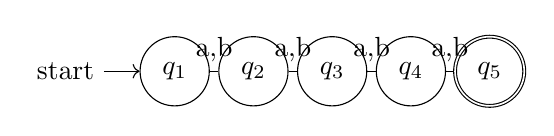
\begin{tikzpicture}
  	\node[state, initial] (q1) {$q_1$};
  	\node[state, right of=q1] (q2) {$q_2$};
  	\node[state, right of=q2] (q3) {$q_3$};
  	\node[state, right of=q3] (q4) {$q_4$};
  	\node[state, accepting, right of=q4] (q5) {$q_5$};
  	\draw
  	(q1) edge[above] node{a,b} (q2)
  	(q2) edge[above] node{a,b} (q3)
  	(q3) edge[above] node{a,b} (q4)
	 (q4) edge[above] node{a,b} (q5)
  	;
  \end{tikzpicture}

  \item \textbf{The language of all words that begin or end with a double letter.}
    \\
  Regular Expression: $(aa+bb)(a+b)\kleene(aa+bb)$
  \\
  Definition: 
  \begin{itemize}
  	\item Finite set of States: $Q = \{1,2,3,4\}$
  	\item Finite set of Symbols in the Language: $\Sigma = \{a,b\}$
  	\item Transition Function: $\delta$
  	\item Initial State: $\{1\}$
  	\item Final State: $\{4\}$
  \end{itemize}
  
  State Diagram:\\
  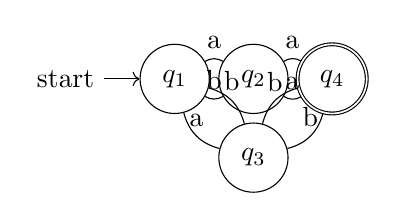
\begin{tikzpicture}
  	\node[state, initial] (q1) {$q_1$};
  	\node[state, right of=q1] (q2) {$q_2$};
  	\node[state, below of=q2] (q3) {$q_3$};
  	\node[state, accepting, right of=q2] (q4) {$q_4$};
  	\draw
  	(q1) edge[bend left, above] node{a} (q2)
  	(q2) edge[bend left, above] node{b} (q1)
  	(q2) edge[bend left, above] node{a} (q4)
  	 (q4) edge[bend left, above] node{a} (q2)
  	(q1) edge[bend left, above] node{b} (q3)
(q3) edge[bend left, above] node{a} (q1)
  	(q3) edge[bend left, above] node{b} (q4)
(q4) edge[bend left, above] node{b} (q3)
  	;
  \end{tikzpicture}
  
  \item \textbf{The language of all words with only $a$'s or only $b$'s. For clarification, the empty string is not in this language.}
  \\
  Regular Expression: $aa\kleene + bb\kleene$
  \\
    Definition: 
  \begin{itemize}
  	\item Finite set of States: $Q = \{1,2,3\}$
  	\item Finite set of Symbols in the Language: $\Sigma = \{a,b\}$
  	\item Transition Function: $\delta$
  	\item Initial State: $\{1\}$
  	\item Final State: $\{2,3\}$
  \end{itemize}
  
  State Diagram:\\
  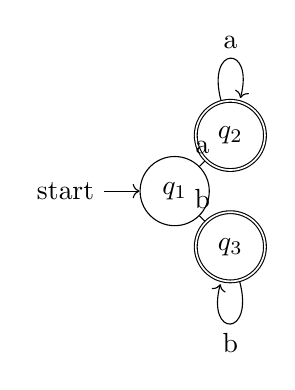
\begin{tikzpicture}
	\node[state, initial] (q1) {$q_1$};
	\node[state, accepting, above right of=q1] (q2) {$q_2$};
	\node[state, accepting, below right of=q1] (q3) {$q_3$};
	\draw

	(q1) edge[above] node{a} (q2)
		(q1) edge[above] node{b} (q3)
	(q2) edge[loop above] node{a} (q2)
	(q3) edge[loop below] node{b} (q3)
	;
\end{tikzpicture}
\end{enumerate}


\newpage
\item \textbf{One of the defining properties of regular languages is that they're recognized by DFAs.}
\begin{enumerate}
  \item Write "every regular language can be recognized by some DFA" as a first-order formula, and find its complement, contrapositive, and dual. Express each of these as both a first-order formula and a written description in English. Hint: for this example, you can treat "can be recognized by some DFA" as a simple predicate.
  \item What can we infer about nonregular languages from this?
  \item What if we didn't treat "can be recognized by some DFA" as a predicate, but instead wrote it as its own expression in first-order logic?
\end{enumerate}
		
\end{enumerate}

% %\bibliography{bibfile}

\end{document}

